
Datorita faptului ca o placa video trebuie sa execute miliarde de calcule matematice, ray traceing,
etc, acesa arhitectura este optimizata pentru acest timp de calcule. Datorita acestui lucru, toate placile
video care sunt compatibile cu tehnologii de tip Cuda sau OpenCL, tehnologii ce pot acelera calcule matematice, in
special lucrul cu matrici. Viteza cu care aceste operatii sunt executate este motivul pentru care
toate super calculatoarele construite in ultimi 5 ani au, pe langa mii de procesoare clasice, si
placi video profesionale. Diferenta intre o placa video profesionala si una clasica este ca aceasta
poate sa execute si operatii matematice in virgula mobila - Figura 4.1. Mai bine zis, pe langa operatii
matematice cu operatori de tip float, aceasta poate accelera foarte bine si operatii matematice cu operatori de
tip double.

Dupa cum se poate observa in testul de mai jos, Fig 4.1, performanta teoretica a placilor video se dubleaza
odata la fiecare an, fata de procesoarele clasice care dubleaza peformanta odata la circa 2-3 ani
de zile. Deasemenea, pe langa performanta imbunatatita, eficienta energetica este si ea din ce in
ce mai buna, iar datele din Figura 4.2, obtinuta dintr-o prezentare Nvidia, demonstreaza acest lucru . 

\begin{figure*}[ht] \centering
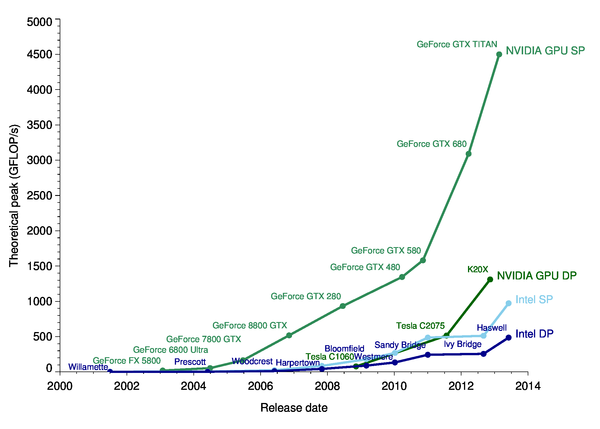
\includegraphics[width=0.9\textwidth]{img/gpu.png}
\caption{Performanta placilor grafice comparativ cu cea a procesoarelor} \end{figure*}


Putem compara si putera placilor video, care, a tot scazut in conditiile in care perfomanta a
crescut. Astfel, Nvidia GTX 580, placa cu arhitectura Fermi, are un consum de 244 de Watti\cite{580}, Nvidia GTX 680,
are un consum de 194 Watti\cite{680}, iar Nvidia GTX 980 are un consum de 165 Watti, in conditiile in care
numarul de Nuclee Cuda a crescut de la 512 la 1536, ajung la GTX 980 sa fie in numar de 2048
\cite{980}.

\begin{figure*}[ht] \centering
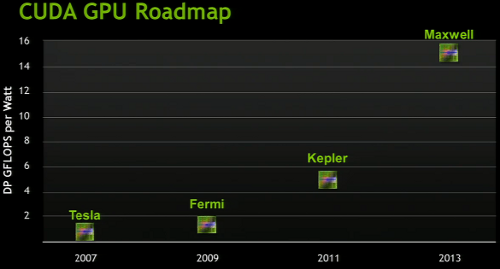
\includegraphics[width=0.9\textwidth]{img/fermi.png}
\caption{Eficienta arhitecturiilor Fermi, Kepler si Maxwell} \end{figure*}


